\fancyhead[RO]{\fontsize{8.5pt}{10pt}\selectfont\textsf{MỤC 1.3}\quad \textsf{Các hàm số mới từ các hàm số cũ}\quad \textbf{\textsf{41}}}

\noindent
\begin{minipage}[t]{0.265\textwidth}
    \fontsize{8pt}{10pt}\selectfont
    \vspace*{24pt}
    \begin{center}
        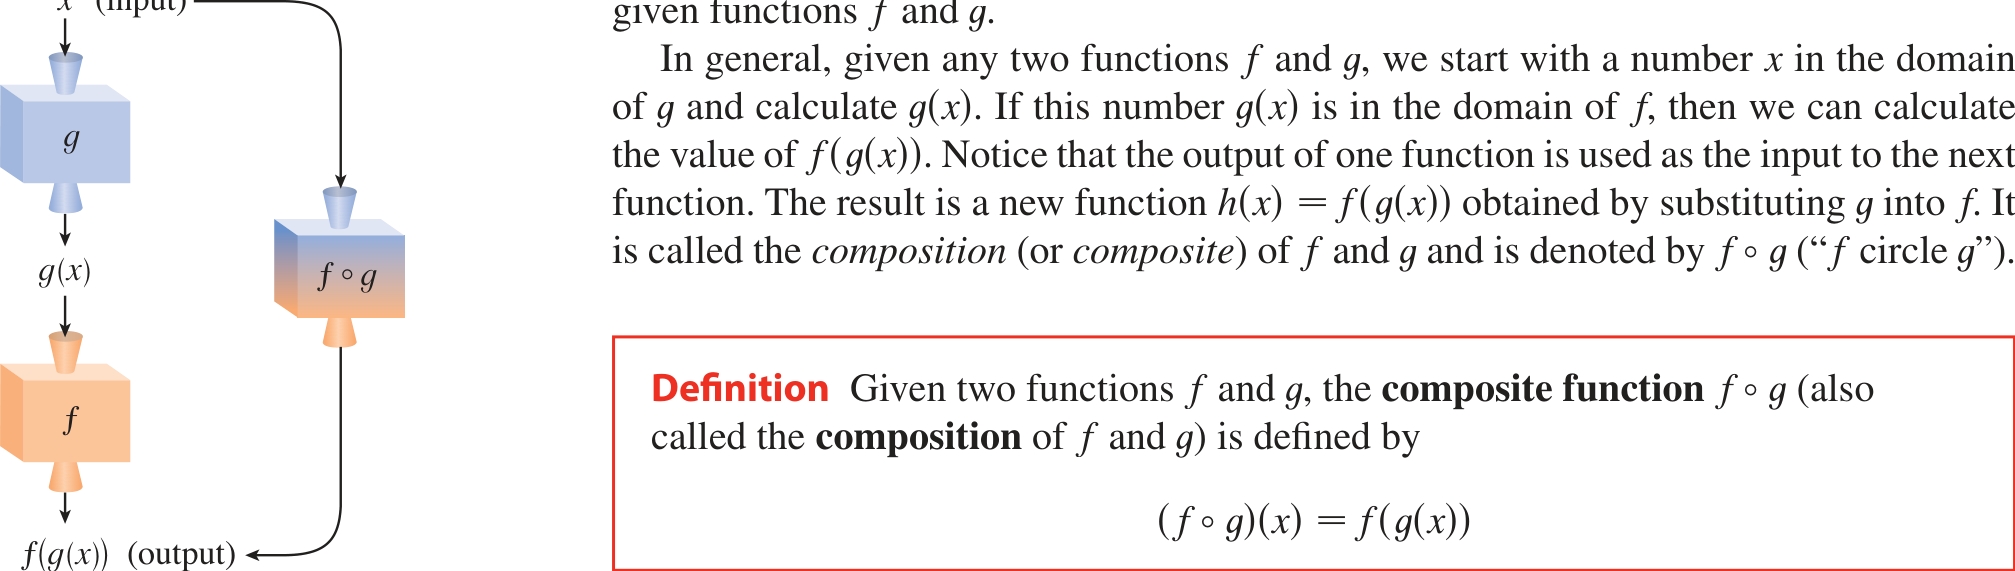
\includegraphics[width=0.92\linewidth]{images/p0076_fig11.png}
    \end{center}
    \vspace{-4pt}
    \textbf{\textsf{HÌNH 11}}\\[2pt]
    Cỗ máy $f \circ g$ được hợp thành từ cỗ máy $g$ (trước) và sau đó là cỗ máy $f$.

    \vspace{210pt}
    \begin{flushright}
        \color{stewartcyan}\textit{Nếu $0 \leqslant a \leqslant b$ thì $a^2 \leqslant b^2$.}
    \end{flushright}
\end{minipage}%
\hfill
\begin{minipage}[t]{0.708\textwidth}
    \fontsize{9.3pt}{13.2pt}\selectfont
    của $u$ và đến lượt $u$ lại là một hàm số của $x$, suy ra rằng rốt cuộc $y$ là một hàm số của $x$. Ta tính điều này bằng phép thế:
    \[
    y = f(u) = f(g(x)) = f(x^2 + 1) = \sqrt{x^2 + 1}
    \]
    Quy trình này được gọi là \textit{phép hợp thành} (composition) bởi vì hàm số mới được \textit{hợp thành} (composed) từ hai hàm số $f$ và $g$ đã cho.

    Nói chung, cho hai hàm số $f$ và $g$ bất kỳ, ta bắt đầu với một số $x$ thuộc tập xác định của $g$ và tính $g(x)$. Nếu số $g(x)$ này thuộc tập xác định của $f$, thì ta có thể tính được giá trị $f(g(x))$. Chú ý rằng kết quả đầu ra của hàm số thứ nhất được sử dụng làm đầu vào cho hàm số tiếp theo. Kết quả thu được là một hàm số mới $h(x) = f(g(x))$ bằng cách thế $g$ vào $f$. Nó được gọi là \textit{hàm hợp} (hay \textit{hợp thành}) của $f$ và $g$, ký hiệu là $f \circ g$ (đọc là ``$f$ hợp $g$'').

    \begin{definitionbox}
        \textbf{\textcolor{stewartred}{Định nghĩa}}\quad Cho hai hàm số $f$ và $g$, \textbf{hàm hợp} $f \circ g$ (còn gọi là \textbf{hợp thành} của $f$ và $g$) được định nghĩa bởi
        \[
        (f \circ g)(x) = f(g(x))
        \]
    \end{definitionbox}

    Tập xác định của $f \circ g$ là tập hợp tất cả các giá trị $x$ thuộc tập xác định của $g$ sao cho $g(x)$ thuộc tập xác định của $f$. Nói cách khác, $(f \circ g)(x)$ xác định bất cứ khi nào cả $g(x)$ và $f(g(x))$ đều xác định. Hình 11 minh họa cách hình dung $f \circ g$ dưới dạng các cỗ máy.

    \vspace{4pt}
    \noindent\textbf{\textsf{\color{stewartcyan}VÍ DỤ 6}}\quad Nếu $f(x) = x^2$ và $g(x) = x - 3$, hãy tìm các hàm hợp $f \circ g$ và $g \circ f$.

    \vspace{2pt}
    \noindent\textbf{\textsf{\color{stewartcyan}LỜI GIẢI}}\quad Ta có
    \begin{align*}
        (f \circ g)(x) &= f(g(x)) = f(x - 3) = (x - 3)^2\\[3pt]
        (g \circ f)(x) &= g(f(x)) = g(x^2) = x^2 - 3
    \end{align*}
    \hfill{\color{stewartcyan}$\blacksquare$}

    \vspace{2pt}
    \noindent\tikz[baseline=-0.7ex]{\draw[stewartred, line width=1pt] (0,0) circle (5.5pt); \draw[stewartred, line width=1pt] (-3.8pt,-3.8pt) -- (3.8pt,3.8pt);}\;\textbf{\textsf{\color{stewartgreen}CHÚ Ý}}\quad Từ Ví dụ 6, bạn có thể thấy rằng nói chung $f \circ g \ne g \circ f$. Hãy nhớ rằng, \textcolor{stewartred}{ký hiệu $f \circ g$ có nghĩa là hàm $g$ được thực hiện trước rồi hàm $f$ mới được thực hiện sau.} Trong Ví dụ 6, $f \circ g$ là hàm số \textit{trước tiên} trừ đi 3 và \textit{sau đó} mới bình phương; còn $g \circ f$ là hàm số \textit{trước tiên} bình phương và \textit{sau đó} mới trừ đi 3.

    \vspace{6pt}
    \noindent\textbf{\textsf{\color{stewartcyan}VÍ DỤ 7}}\quad Nếu $f(x) = \sqrt{x}$ và $g(x) = \sqrt{2 - x}$, hãy xác định từng hàm số sau cùng tập xác định của nó:
    \begin{center}
        \textbf{(a)}\; $f \circ g$ \qquad\qquad \textbf{(b)}\; $g \circ f$ \qquad\qquad \textbf{(c)}\; $f \circ f$ \qquad\qquad \textbf{(d)}\; $g \circ g$
    \end{center}

    \vspace{-2pt}
    \noindent\textbf{\textsf{\color{stewartcyan}LỜI GIẢI}}

    \noindent\textbf{(a)}\;
    \[
    (f \circ g)(x) = f(g(x)) = f(\sqrt{2 - x}) = \sqrt{\sqrt{2 - x}} = \sqrt[4]{2 - x}
    \]
    Tập xác định của $f \circ g$ là $\{x \mid 2 - x \geqslant 0\} = \{x \mid x \leqslant 2\} = (-\infty, 2]$.

    \vspace{3pt}
    \noindent\textbf{(b)}\;
    \[
    (g \circ f)(x) = g(f(x)) = g(\sqrt{x}) = \sqrt{2 - \sqrt{x}}
    \]
    Để $\sqrt{x}$ xác định, ta phải có $x \geqslant 0$. Để $\sqrt{2 - \sqrt{x}}$ xác định, ta phải có $2 - \sqrt{x} \geqslant 0$, tức là $\sqrt{x} \leqslant 2$, hay $x \leqslant 4$. Do đó ta có $0 \leqslant x \leqslant 4$, vậy tập xác định của $g \circ f$ là đoạn $[0, 4]$.

    \vspace{3pt}
    \noindent\textbf{(c)}\;
    \[
    (f \circ f)(x) = f(f(x)) = f(\sqrt{x}) = \sqrt{\sqrt{x}} = \sqrt[4]{x}
    \]
    Tập xác định của $f \circ f$ là $[0, \infty)$.
\end{minipage}